\documentclass{book}
\usepackage{blindtext}
\usepackage{geometry}
 \geometry{
 a4paper,
 total={170mm,257mm},
 left=30mm,
 right=30mm,
 top=26mm,
 bottom=35mm,
 }
\usepackage{graphicx}
\graphicspath{ {images/} }
\usepackage{float}
\usepackage{wrapfig}
\usepackage[utf8]{inputenc}
\usepackage[english,russian]{babel}
\usepackage[T2A]{fontenc}
\usepackage{mathtools}
\usepackage{amssymb}
\usepackage{fancyhdr}
\pagestyle{fancy}
\fancyhf{}

\begin{document}

\cfoot{\fontsize{15,8pt}{15pt}\selectfont{\stackrel{\line(1,0){70}}{\textit{37}}}}
\renewcommand{\headrulewidth}{0pt}
{\fontsize{15,8pt}{18pt}\selectfont
I$_{3}$. \textit{Существует число, обозначаемое $0$ и называемое нулем,
такое, что для любого числа $a$}
$$
a + 0 = a.
$$}

{\fontsize{15,8pt}{18pt}\selectfont
I$_{4}$. \textit{Для любого числа $a$ существует число, обозначаемое $-a$ и 
называемое противоположным данному, такое, что}
$$
a + (-a) = 0.
$$}

{\fontsize{15,8pt}{18pt}\selectfont
ІІ. О\ п\ е\ р\ а\ ц\ и\ я\ \ у\ м\ н\ о\ ж\ е\ н\ и\ я. Для любой упорядоченной пары чисел $a$ и $b$
 определено, и притом единственным образом, число, называемое их \textit{произведением} и
обозначаемое
$ab$ (или $a\cdot b$), так что при этом имеют место следующие свойства.}

{\fontsize{15,8pt}{18pt}\selectfont
II$_{1}$. \textit{Для любой пары чисел $a$ и $b$}
$$
ab = ba.
$$
Это свойство называется \textit{переместительным} или \textit{коммутативным законом умножения.}}

{\fontsize{15,8pt}{18pt}\selectfont
II$_{2}$. \textit{Для любых чисел $a$, $b$, $c$}
$$
a(bc) = (ab)c.
$$
Это свойство называется \textit{сочетательным} или \textit{ассоциативным законом умножения.}}

{\fontsize{15,8pt}{18pt}\selectfont
II$_{3}$. \textit{Существует число, обозначаемое} 1 \textit{и называемое единицей, 
такое, что для любого числа $a$}
$$
a\cdot 1 = a.
$$}

{\fontsize{15,8pt}{18pt}\selectfont
II$_{4}$. \textit{Для любого числа $a\ne 0$ существует число, обозначаемое $1/a$ 
или $\frac{1}{a}$ и называемое
обратным данному, такое, что}
$$
a\cdot\frac{1}{a} = 1.
$$}

{\fontsize{15,8pt}{18pt}\selectfont
ІІІ. С\ в\ я\ з\ ь\ \ о\ п\ е\ р\ а\ ц\ и\ й\ \ с\ л\ о\ ж\ е\ н\ и\ я\ \ и\ \ у\ м\ н\ о\ ж\ е\ н\ и\ я. 
\textit{Для любых чисел $a$, $b$, $c$}
$$
(a + b)c = ac + bc.
$$
Это свойство называется \textit{распределительным} или \textit{дистрибутивным 
законом умножения} относительно сложения.}

{\fontsize{15,8pt}{18pt}\selectfont
ІV. У\ п\ о\ р\ я\ д\ о\ ч\ е\ н\ н\ о\ с\ т\ ь. \textit{Для каждого числа $a$ определено 
одно из соотношений
$a > 0$ (а больше нуля), $a = 0$}}

\newpage
\cfoot{\fontsize{15,8pt}{18pt}\selectfont{\stackrel{\line(1,0){70}}{\textit{38}}}}
\renewcommand{\headrulewidth}{0pt}

\begin{figure}[!h]



	\left{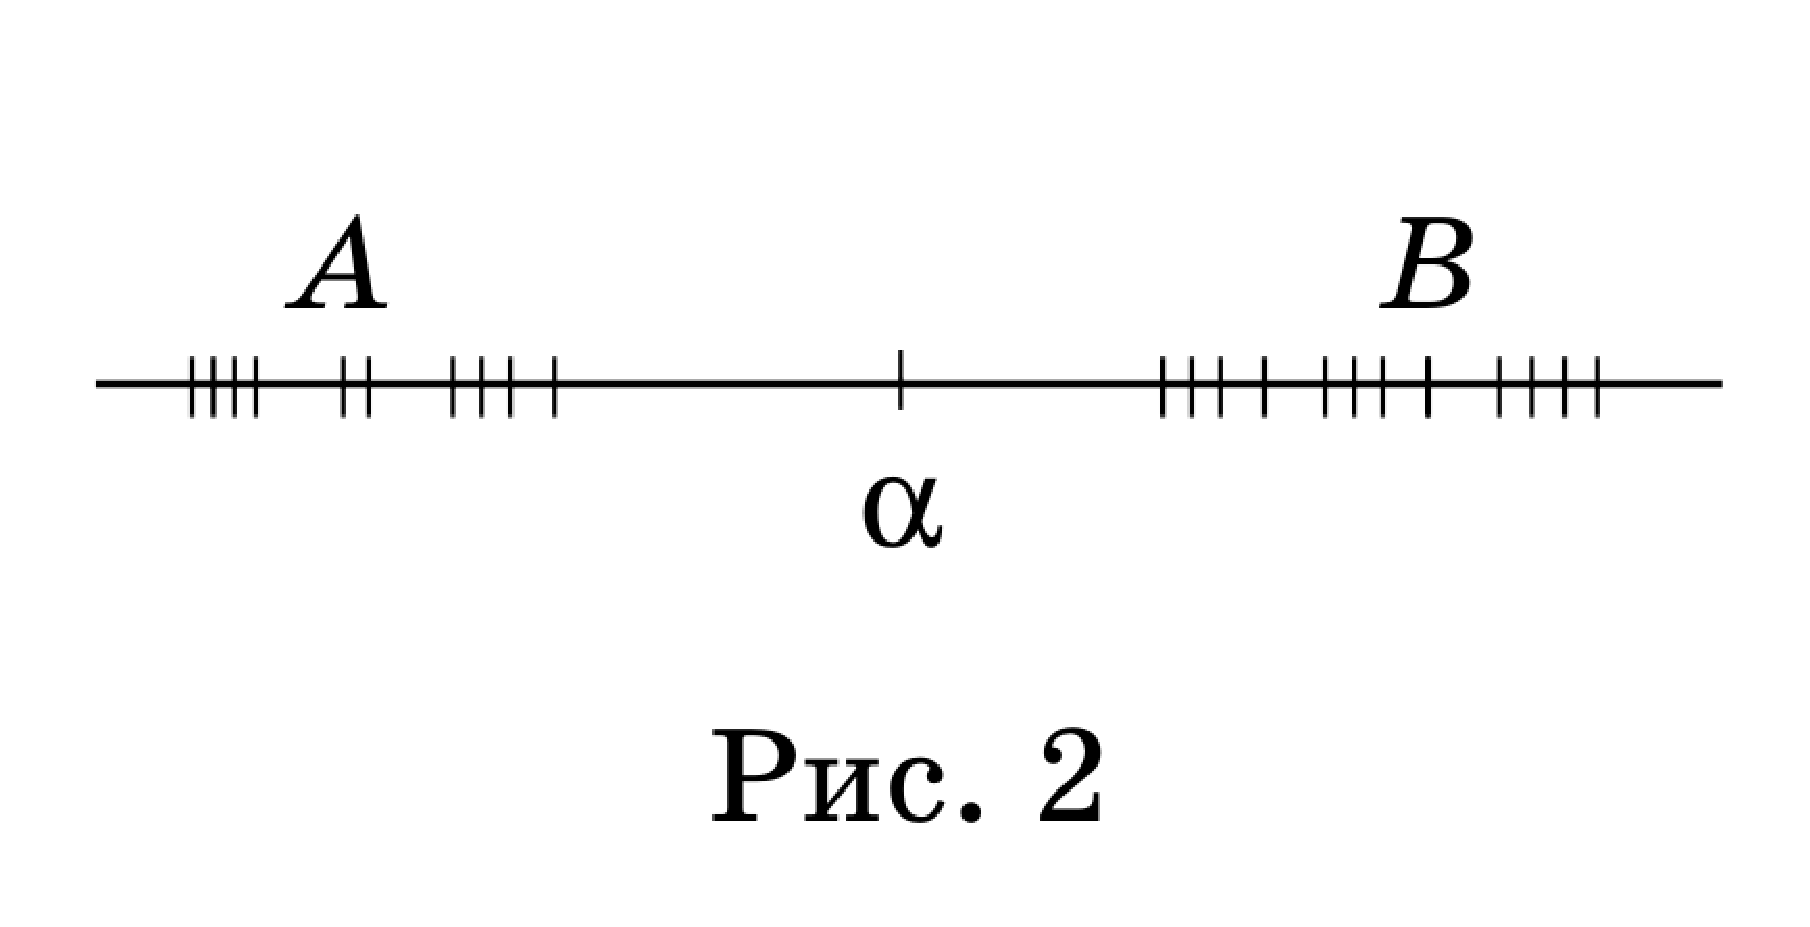
\includegraphics[width=0.4\linewidth]{рисунок(1).eps}}\box{\begin{minipage}{0.55\textwidth}
	{\fontsize{15,8pt}{18pt}\selectfont
        \textit{($a$ равно нулю) или $a < 0$ ($a$ меньше нуля) так, что условие 
        $a > 0$ равносильно условию $-a < 0$.}}

        {\fontsize{15,8pt}{18pt}\selectfont
        \textit{При этом если $a > 0$, $b > 0$, то имеют место неравенства:}}
\end{minipage}}
\end{figure}

{\fontsize{15,8pt}{18pt}\selectfont
IV$_{1}$. $a + b > 0$.}

{\fontsize{15,8pt}{18pt}\selectfont
IV$_{2}$. $ab > 0$.}

{\fontsize{15,8pt}{18pt}\selectfont
Свойство ІV дает возможность ввести понятие сравнения или, 
как иногда говорят, сравнения по величине для любых двух чисел.}

{\fontsize{15,8pt}{18pt}\selectfont
Число $b$ называют числом, б\'{о}льшим числа $a$, и пишут $b > a$, или, что то же самое, 
число $a$ называют меньшим числа $b$ и пишут $a < b$, если $b - a > 0$.}

{\fontsize{15,8pt}{18pt}\selectfont
Наличие сравнения <<больше>> или <<меньше>> для любой пары действительных чисел 
называется \textit{свойством упорядоченности множества всех действительных чисел.}}

{\fontsize{15,8pt}{18pt}\selectfont
Действительные числа обладают еще так называемым
свойством непрерывности.}

{\fontsize{15,8pt}{18pt}\selectfont
V. С\ в\ о\ й\ с\ т\ в\ о\ \ н\ е\ п\ р\ е\ р\ ы\ в\ н\ о\ с\ т\ и. \textit{Каковы бы ни бы ли непустые множества 
$A\subset\textbf{R}$ и $B\subset\textbf{R}$, у которых для любых двух элементов 
$a\in A$ и $b\in B$ выполняется неравенство $a\leqslant b$, существует такое число $\alpha$, 
что для всех $a\in A$ и $b\in B$ имеет место} (рис. 2) \textit{соотношение}
$$
a\leqslant\alpha\leqslant b.
$$}

{\fontsize{15,8pt}{18pt}\selectfont
Свойство непрерывности действительных чисел связано с самым простейшим 
использованием математики на практике --- с измерением величин. При измерении 
какой-либо физической или какой-нибудь другой природы величины часто получают 
с большей или меньшей точностью ее приближенные значения. Если в результате 
экспериментального измерения данной величины получается ряд чисел, дающих 
значение искомой величины с недостатком (они играют роль множества $А$ в 
приведенной выше формулировке свойства непрерывности) и с избытком (множество $В$), 
то свойство непрерывности действительных чисел выражает объективную уверенность 
в том, что измеряемая величина имеет определенное значение, расположенное между 
ее приближенными значениями, вычисленными с недостатком и избытком.
}

{\fontsize{15,8pt}{18pt}\selectfont
Из свойств I---V действительных чисел вытекают другие многочисленные их свойства, 
поэтому можно сказать, что действительные числа представляют собой совокупность 
элементов, обладающую свойствами I---V.}

\end{document}
